\midheading{$Z\gamma$, production, processes 300, 305}
\label{subsec:zgamma}


Processes {\tt 300} and {\tt 305} represent the production of a $Z$ boson (or virtual photon for process {\tt 300})
in association with a real photon based on ref.~\cite{Campbell:2017aul}. The $Z/\gamma^*$ subsequently decays into
either an $e^+ e^-$ pair ({\tt nproc=300}) or neutrinos ({\tt nproc=305}).
Since these processes include a real photon, the cross section diverges
when the photon is very soft or in the direction of the beam.
Thus in order to produce sensible results, the input file must supply values for both
{\tt gammptmin} and {\tt gammrapmax}. Moreover, when the parameters {\tt zerowidth}
and {\tt removebr} are set to {\tt .false.} the decay $Z \to e^- e^+$ ({\tt nproc=300})
will include photon radiation from both leptons, so that a non-zero $R(\gamma,\ell)_{min}$
({\tt Rgalmin})
should also be supplied. This will ensure that the cross section is well-defined.
The calculation of processes {\tt 300} may be performed
at NNLO using the Frixione algorithm~\cite{Frixione:1998jh} or standard isolation.
The one-loop virtual diagrams are taken from \cite{Dixon:1998py} and the two-loop virtual diagrams
are taken from \cite{Gehrmann:2011ab}.

%Processes {\tt 302} and {\tt 307}  represents the production of a $Z$ boson (or virtual photon)
%in association with a real photon and an additional jet. These processes are also available at NLO including
%the full fragmentation processes. Anomalous couplings are not available for these processes.
%Processes {\tt 304} and {\tt 309}  represents the production of a $Z$ boson (or virtual photon)
%in association with a real photon and and two additional jets. These processes are available at leading order only.
%When {\tt removebr} is true in process {\tt 300} or {\tt 302} the $Z$ boson does not decay.

For the process {\tt 300}  the role of {\tt mtrans34cut} changes to become a cut
on the invariant mass on the $M_{345}$ system, i.e. the photon is included with the leptons in the cut.

\bottomheading{Anomalous $ZZ\gamma$ and $Z\gamma\gamma$ couplings}
Processes {\tt 300}-{\tt 305} may also be computed including the effect of anomalous couplings between $Z$ bosons and 
photons.
Note that, at present, the effect of anomalous couplings is not included in the gluon-gluon
initiated contributions.

The anomalous $Z\gamma Z$ vertex (not present at all in the Standard Model),
considering operators up to dimension 8, is given by~\cite{DeFlorian:2000sg},

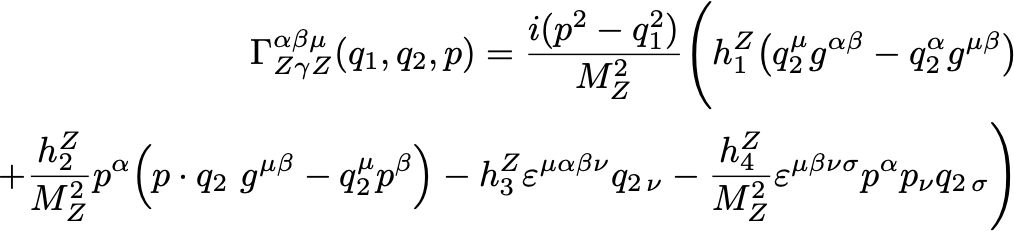
\includegraphics[width=0.9\textwidth]{./sections/gobbets/ZZgamma.png}
%\begin{eqnarray}
% && \Gamma^{\alpha \beta \mu}_{Z \gamma Z}(q_1, q_2, p) = 
%   \frac{i(p^2-q_1^2)}{M_Z^2} \Biggl( 
%   h_1^Z \bigl( q_2^\mu g^{\alpha\beta} - q_2^\alpha g^{\mu \beta}
%   \bigr) \nonumber \\
%&& + \frac{h_2^Z}{M_Z^2} p^\alpha \Bigl( p\cdot q_2\ g^{\mu\beta} -
%            q_2^\mu p^\beta \Bigr)
%   - h_3^Z \varepsilon^{\mu\alpha\beta\nu} q_{2\, \nu} 
%   - \frac{h_4^Z}{M_Z^2} \varepsilon^{\mu\beta\nu\sigma} p^\alpha
%p_\nu q_{2\, \sigma} \Biggl)
%\end{eqnarray}

where the overall coupling has been chosen to be $|e|$ (and
$\epsilon^{0123}=+1$). The non-standard $Z_\alpha(q_1) \gamma_\beta(q_2)
\gamma_\mu(p)$ momentum-space vertex can be obtained from
this equation by setting $q_1^2 \to 0$ and replacing $h_i^Z \to
h_i^\gamma$. 
The parameters that
specify the anomalous couplings, $h_i^Z$ and $h_i^\gamma$ (for $i=1\ldots 4$), are
specified in the input file as, e.g. {\tt h1(Z)} and {\tt h1(gamma)}.
If the input file contains a negative value for the form-factor scale $\Lambda$
then no suppression factors are applied to these anomalous couplings.
Otherwise, the couplings are included
in MCFM only after suppression by dipole form factors,
\begin{equation}
h_{1,3}^{Z/\gamma} \rightarrow
 \frac{h_{1,3}^{Z/\gamma}}{(1+\hat{s}/\Lambda^2)^3}, \qquad
h_{2,4}^{Z/\gamma} \rightarrow
 \frac{h_{2,4}^{Z/\gamma}}{(1+\hat{s}/\Lambda^2)^4}, \qquad
\end{equation}
where $\hat{s}$ is the $Z\gamma$ pair invariant mass. Note that these form factors are slightly
different from those discussed in Sections~\ref{subsec:diboson} and~\ref{subsec:wgamma}. The
form factors can be modified in {\ttfamily src/Need/set\_anomcoup.f}.

The Standard Model cross section is obtained by setting $h_i^Z = h_i^\gamma = 0$ for $i=1\ldots 4$.
